\documentclass[a4paper]{article}

\usepackage{amssymb}
\usepackage[shortlabels]{enumitem}
\usepackage{indentfirst}

\usepackage{listings}

\usepackage{float}
\floatstyle{plaintop}
\restylefloat{table}

\usepackage{caption} 
\captionsetup[table]{skip=10pt}

\captionsetup[table]{skip=10pt}

\lstdefinestyle{mystyle}{
    basicstyle=\ttfamily\footnotesize,
    breakatwhitespace=false,
    breaklines=true,
    captionpos=b,
    keepspaces=true,
    showspaces=false,
    showstringspaces=false,
    showtabs=false,
    tabsize=2
}
\lstset{style=mystyle}


\title{
    Data Structure Review: Graphs\\
}

\author{
    \small{Author: Francisco Ricardo Taborda Aguiar}\\
}

\date{\today}

\begin{document}

    \maketitle


    \section{Overview}

    TODO:
    história
    aplicações práticas (enfatizar neo4j)
        networks (ideal ds for modeling networks), social networks
        The applications of graphs include finding the shortest path, 
        finding the best starting point, breadth-first and depth-first 
        traversal, searching, inserting, deleting from a tree or 
        linked list, graph classification, finding missing relationships 
        through link prediction, and node classification.

    A graph is a way to represent relationships between pairs 
    of objects \cite{goodrich:2014} or entities.
    A graph can be defined by a set of vertices and a collection 
    of edges. The edges can contain a weight to represent an 
    arbitrary value, such as cost, or distance, or quantify, 
    for example.
    Vertices (also called nodes) represent entities in graphs, 
    whereas edges represent 
    relationships between those entities \cite{xia:2021}.
    In an abstract point of view, a graph \emph{G} is a set of vertex 
    \emph{V} and a collection \emph{E} of pairs of vertex (the edges).

    The graph may be directed, when the edges are ordered pairs 
    \emph{(u, v)} of vertices, with \emph{u} preceding \emph{v}.
    This type of graph is also called digraph.

    The graph is undirected, when the edges are unordered pairs of 
    vertices, also represented as \emph{(u, v)}. In this type of 
    graph, the edge \emph{(u, v)} is identical to the edge 
    \emph{(v, u)}.

    
    The two vertices connected by an edge are called endpoints.
    Adjacent vertices are two vertices that are joined by an edge.
    Adjacent edges are two edges that have an endpoint in common.
    A vertex joined to itself by an edge is called loop.

    An edge is incident to a vertex if the vertex is an endpoint of
    the edge.

    Usually, the edges can be represented by a triplet 
    \emph{(u, v, w)}, with \emph{u} and \emph{v} as 
    the endpoints, and \emph{w} as the weight.

    The degree of a vertex \emph{v} (\emph{deg{v}}) corresponds to 
    the number of the incident edges to the vertex \emph{v}.
    The input degree (\emph{indeg(v)}) of a vertex \emph{v} consists 
    of the number of incident edges in \emph{v}.
    The output degree (\emph{outdeg(v)}) of a vertex \emph{v} is the 
    number of incident edges from \emph{v}.

    If \emph{G} is a graph with \emph{m} edges, then:
    \begin{equation} \label{eq1}
        \sum_{v \in G} deg(v) = 2m
    \end{equation}

    The definition \ref{eq1} is justified by the fact that the dege 
    \emph{(u, v)} is counted twice, one for the endpoint \emph{(u)} and 
    another for the endpoint \emph{(v)}.

    If \emph{G} is a directed graph with \emph{m} edges, then:
    \begin{equation} \label{eq2}
        \sum_{v \in G} indeg(v) = \sum_{v \in G} outdeg(v) = m
    \end{equation}

    In a directed graph one edge \emph{(u, v)} counts as one unit 
    for the output degree of the source \emph{u} and one unit for
    the input degree of the target \emph{v}.

    Let us consider a simple graph with \emph{n} vertices and \emph{m} 
    edges. If \emph{G} is not a directed graph, then:
    \begin{equation} \label{eq3}
        m \le n(n - 1) / 2 
    \end{equation}

    Two edges can not have the same start point and end point and there 
    is no loops. So, a maximum degree of an edge in \emph{G} is $n - 1$. 
    So, by the definition \ref{eq1}:

    \begin{equation} \label{eq4}
        2m = n(n - 1)
    \end{equation}

    Based on the definition \ref{eq2}, the maximum degree of a vertex in \emph{G}
    of a directed graph is:
    \begin{equation}
        m \le n(n-1)
    \end{equation}
    


    A path from vertex \emph{v0} to vertex \emph{vn} is an alternating sequence of 
    vertices and edges $ P =< v_0, e_1, v_1, e_2, ..., v_{n-1}, e_n, v_n > $
    such that the endpoints of $ e_i $ are $ v_{i-1} $, $ v_i $ and there are no 
    repeated edges or vertices (except possibly the initial and final vertices).
    A cycle is a path such that start vertex and end vertex are the same.

    \section{Implementation Strategies}    
    

    The following sections will cover three implementation strategies for graphs.
    The section \ref{edgelist} presents \emph{Edge List}.
    The section \ref{adjacency_matrix} is about \emph{Adjacenty Matrix}.
    The section \ref{adjacency_list} demonstrates \emph{Adjacency List}.


    \begin{figure}[H]
        \centering
        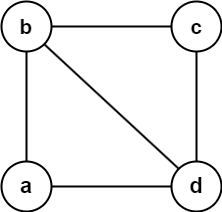
\includegraphics[width=100mm]{images/graphs-undirected.png}
        \vspace*{3mm}
        \caption{Example Graph.}
        \label{graph-algorithm-example}
    \end{figure}


    
    \subsection{Edge List} \label{edgelist}

    The more simple data structure for graphs is Edge List.
    In this particular implementation, a single list of pairs serves as the 
    underlying data structure for storing all the vertices and edges. Each pair 
    represents a single edge and consists of the two distinct identifiers of the 
    vertices it connects. The edge list contains an entry for every line or edge 
    in the graph, and this one data structure stores all the vertices and their 
    relationships. The table \ref{tab:edge-list} 

    \begin{table}[H]
        \centering
        \caption{\label{tab:edge-list}Edge List.}
        \vspace*{10pt}
        \begin{tabular}{ |l|l|l| } 
            \hline
            Index & Vertex 1 & Vertex 2 \\
            \hline
            0   & a & b \\
            \hline
            1   & b & c \\
            \hline
            2   & c & d \\
            \hline
            3   & d & a \\
            \hline
            4   & b & d \\
            \hline            
        \end{tabular}
    \end{table}


    \subsection{Adjacency Matrix} \label{adjacency_matrix}

        
    \begin{table}[H]
        \centering
        \caption{\label{tab:adjacency-matrix}Adjacency Matrix.}
        \vspace*{10pt}
        \begin{tabular}{ l|l|l|l|l|l| } 
                & a & b & c & d \\
            \hline
            a   & 0 & 1 & 0 & 1 \\
            b   & 1 & 0 & 1 & 1 \\
            c   & 0 & 1 & 0 & 1 \\
            d   & 1 & 1 & 1 & 0 \\
            \hline
        \end{tabular}
    \end{table}



    \subsection{Adjacency List} \label{adjacency_list}


    \begin{verbatim}
        { 
            "a": ["b", "d"],
            "b": ["a", "c", "d"],
            "c": ["b", "d"],
            "d": ["a", "b", "c"]
        }
    \end{verbatim}


    \section{Applications}
    TODO


    \section*{Conclusion}
    TODO

    \bibliographystyle{ieeetr}
    \bibliography{graphs} 

\end{document}


https://algodaily.com/lessons/implementing-graphs-edge-list-adjacency-list-adjacency-matrix/java


https://math.libretexts.org/Bookshelves/Combinatorics_and_Discrete_Mathematics/Combinatorics_and_Graph_Theory_(Guichard)/05%3A_Graph_Theory/5.01%3A_The_Basics_of_Graph_Theory